\chapter{Travaux}
  \section{Modélisation}
    \subsection{Modélisation architecturale}
      
      Afin de réaliser la modélisation architecturale c'est AADL\cite{aadl} qui a
      été choisi. AADL, pour {\it Architecture Analysis \& Design Language}, est
      un langage de modélisation d'architectures des sytèmes embarqués et temps
      réel issu de la recherche avionique. De fait, il ne définit pas qu'une
      syntaxe permettant de composer des modèles mais également une sémantique
      qui en fait un outil de modélisation spécifique au domaine de l'embarqué.

      ~

      AADL été conçu originellement en tant qu'un langage textuel. Le but d'une
      telle démarche était de garantir une complète definition de sa syntaxe. De
      fait, il est possible de réaliser des vérifications, des simulations et de
      générer du code source à partir de modèles AADL. Le standard AADL défini
      aujourd'hui trois format de modèles AADL. Un format textuel utile à la
      réalisation de modélisations complètes et détaillées. Un format graphique
      utile au processus de conception et à la documentation. Un format basé sur
      XML utile à l'exploitation des modèles AADL par des outils informatique.

    % TODO Mettre en avant ce qui se retrouve dans la modélisation comportementale
    \subsubsection{Première spécification}

      Il s'agit ici d'une modélisation architecturale basée sur la première
      version des spécifications du démonstrateur. Une modélisation s'appuyant
      sur la seconde version des spécifications sera présentée par la suite.
      
      ~
  
      \begin{figure}[!ht]
        \centering 
        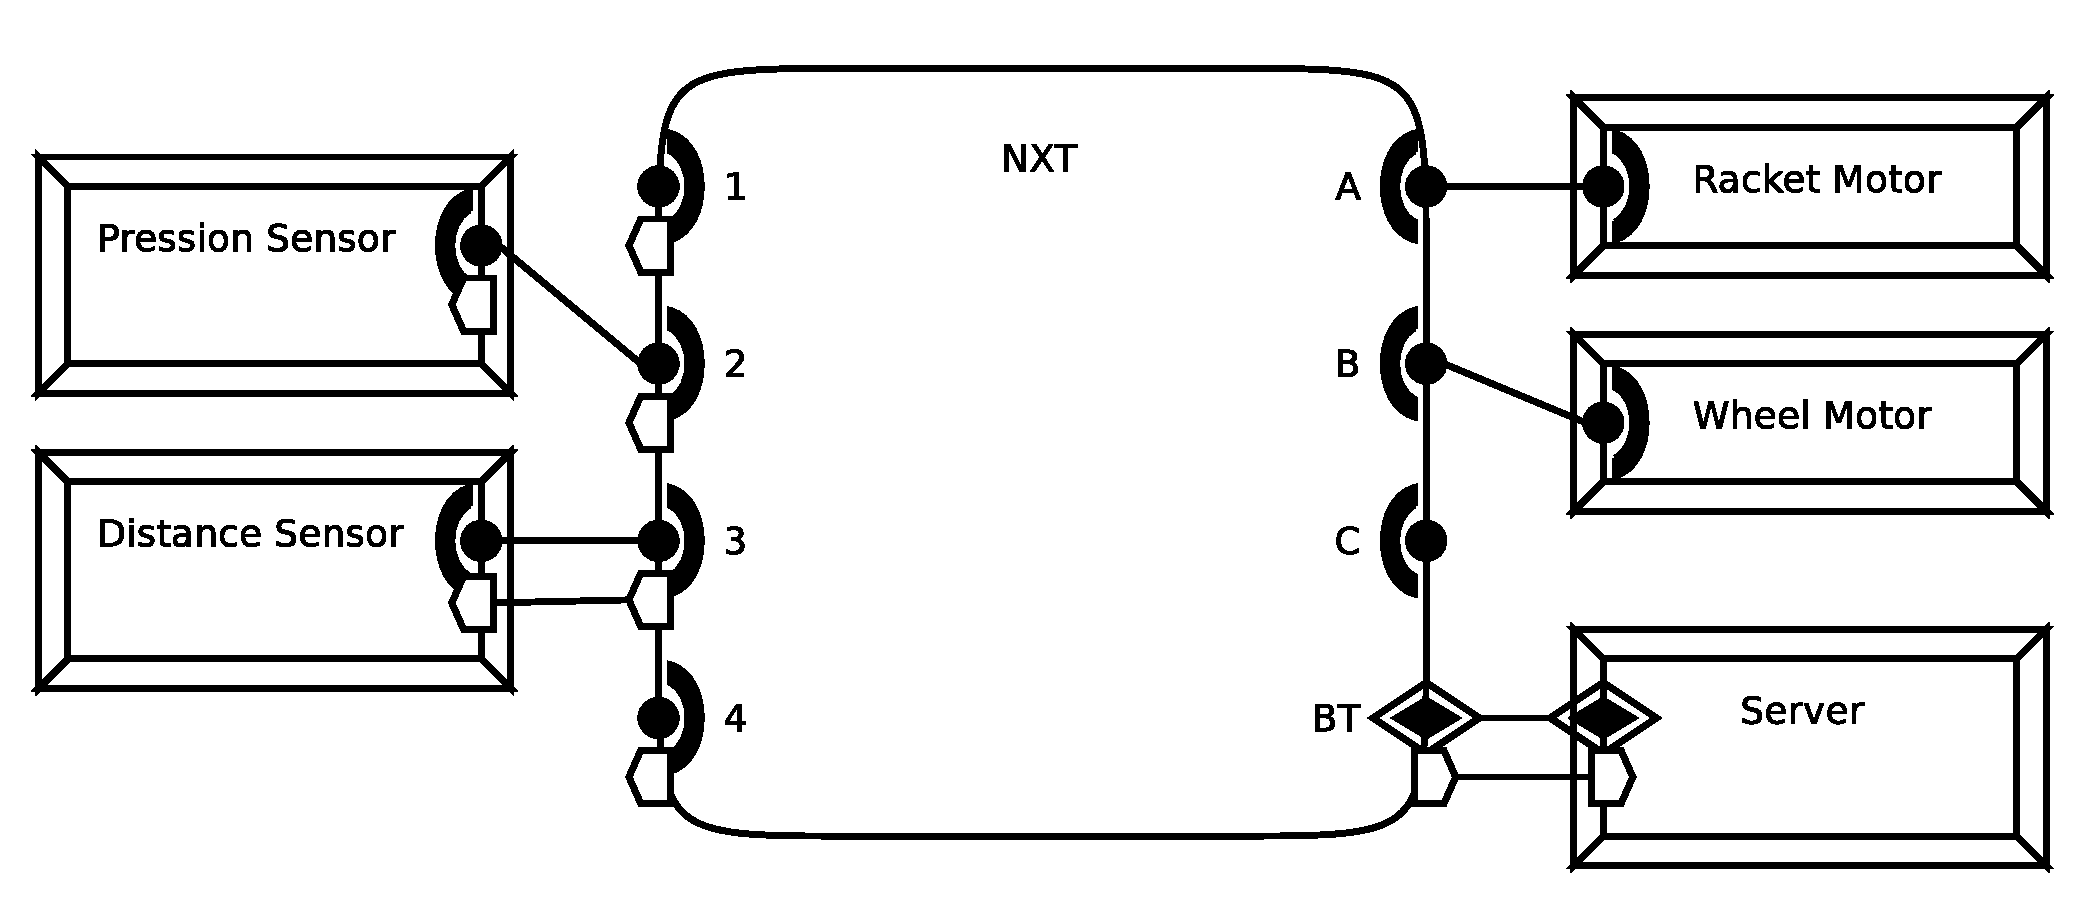
\includegraphics[scale=0.25]{./img/aadl-robot1.pdf}
        \caption{Vue global du système.}
        \label{fig:aadl-robot1}
      \end{figure}
        
      La figure \ref{fig:aadl-robot1} offre une représentation
      graphique du macro-modèle du robot. Le composant principal est
      le système {\it NXT}, les composants l'entourant sont des
      périphériques. Afin de réaliser son positionnement latéral le
      robot est équipé d'un capteur de distance ({\it Distance
        Sensor}), d'une connection à un serveur par {\it bluetooth}
      ({\it Server}) et d'un moteur actionnant une roue ({\it Wheel
        Motor}). Afin de frapper la balle le robot est équipé d'un
      moteur actionnant une raquette ({\it Racket Motor}) ainsi que
      d'un capteur de pression indiquant la fin de course de la
      raquette ({\it Pression Sensor}).

      Le système {\it NXT} est constitué de quatre groupes de ports
      d'entrées indexés de 1 à 4 et de trois groupes de ports de
      sorties indexés de A à C. À ceux-xi s'ajoute un port
      d'entrée/sortie inquiqué par le label BT.

      Le flux de données entre le capteur de pression et le système
      est réalisé par une connection d'entrée/sortie de type {\it digital I/O}.
      Les flux de données entre les deux moteurs et le systèmes sont
      réalisés par des connections à modulation largeur d'impulsion
      ({\it PWM}). Le flux de données et d'évènements entre le capteur
      de distance et le système est réalisé par une connexion sur
      un bus {\it I2C}. Enfin, le flux de données et d'évènements entre le
      serveur et le système est réalisé par une connexion sur un bus {\it
        bluetooth}.

      ~

      \begin{figure}[!ht]
        \centering
        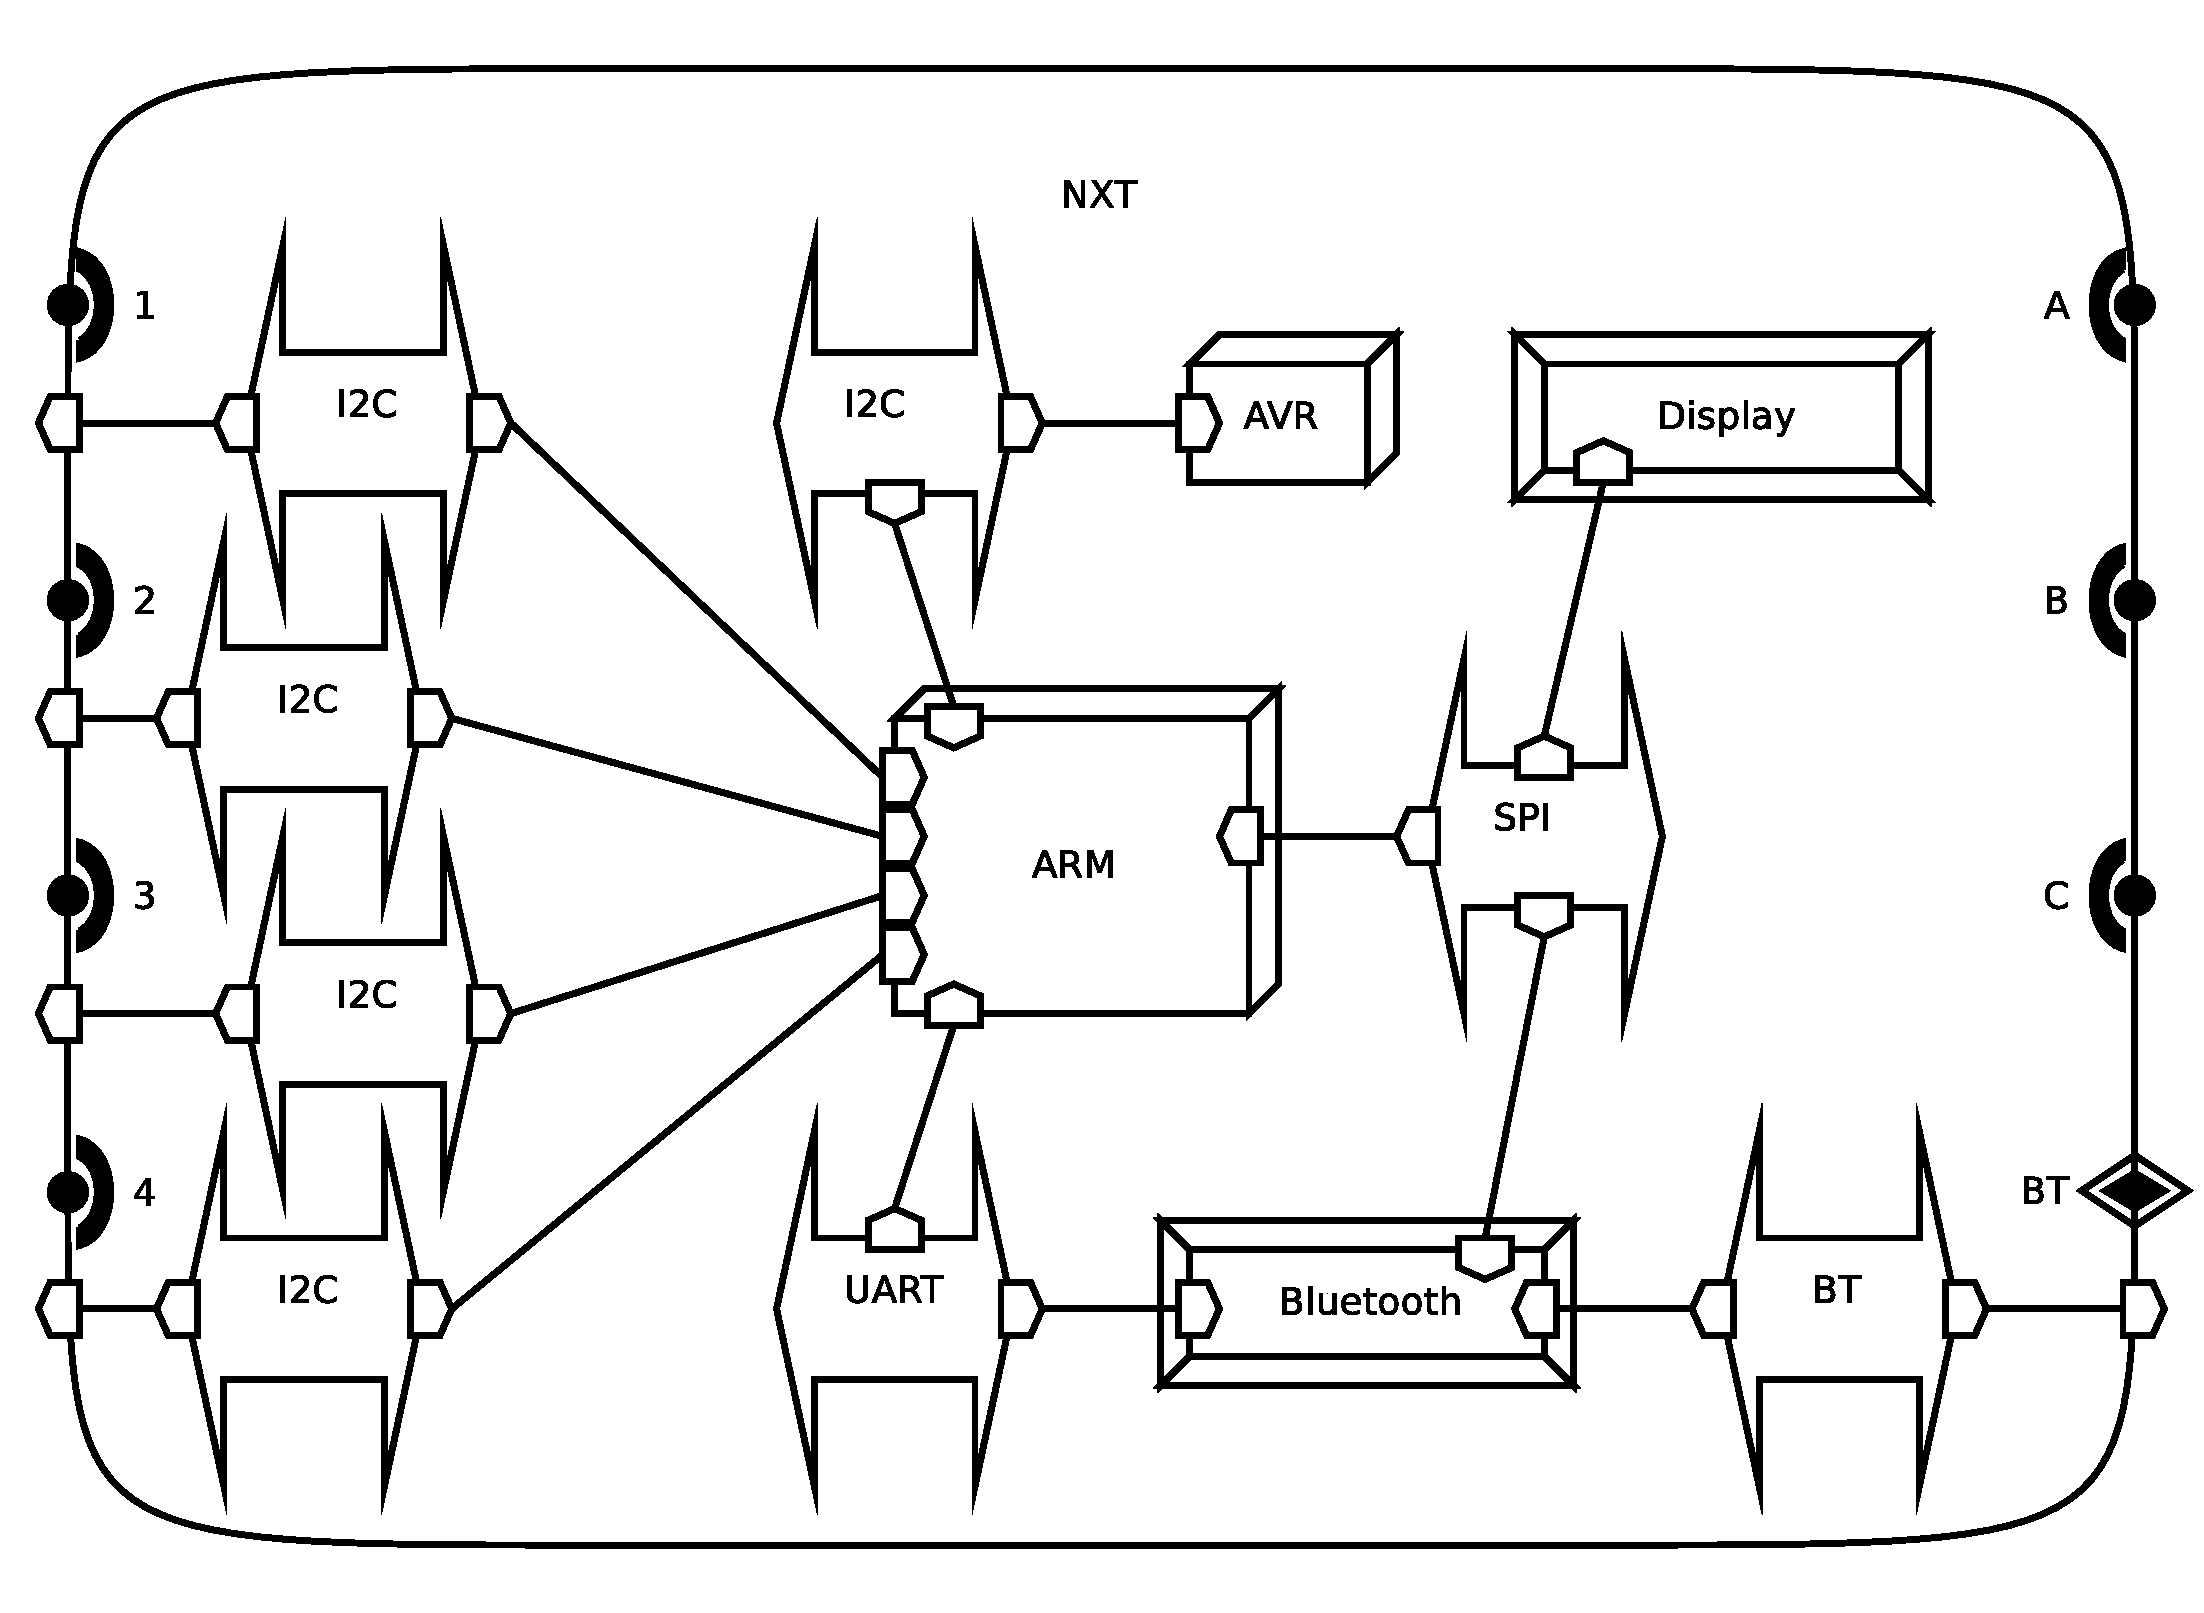
\includegraphics[scale=0.25]{./img/aadl-nxt1h.pdf}
        \caption{Modélisation AADL des composants matériels du NXT.}
        \label{fig:aadl-nxt1h}
      \end{figure}

      La figure \ref{fig:aadl-nxt1h} offre une représentation graphique du
      modèle matériel interne du {\it NXT}. Le composant principal est le
      processeur {\it ARM}, il est accompagné d'un coprocesseur ({\it AVR})
      ainsi que de différents bus et périphériques internes.

      L'ensemble des traitements est réalisés par le processeur. L'interaction
      avec certains périphériques est délégué au coprocesseur notamment avec les
      différents moteurs. Processeur et coprocesseur sont liés par un bus {\it
        I2C}. Le périphérique {\it bluetooth} interne est doublement lié au
      processeur par un bus {\it UART} et un bus {\it SPI}. Les groupes de
      ports d'entrées sont couplé chacun à un bus {\it I2C} qui les relient au
      processeur.

      ~

      \begin{figure}[!ht]
        \centering
        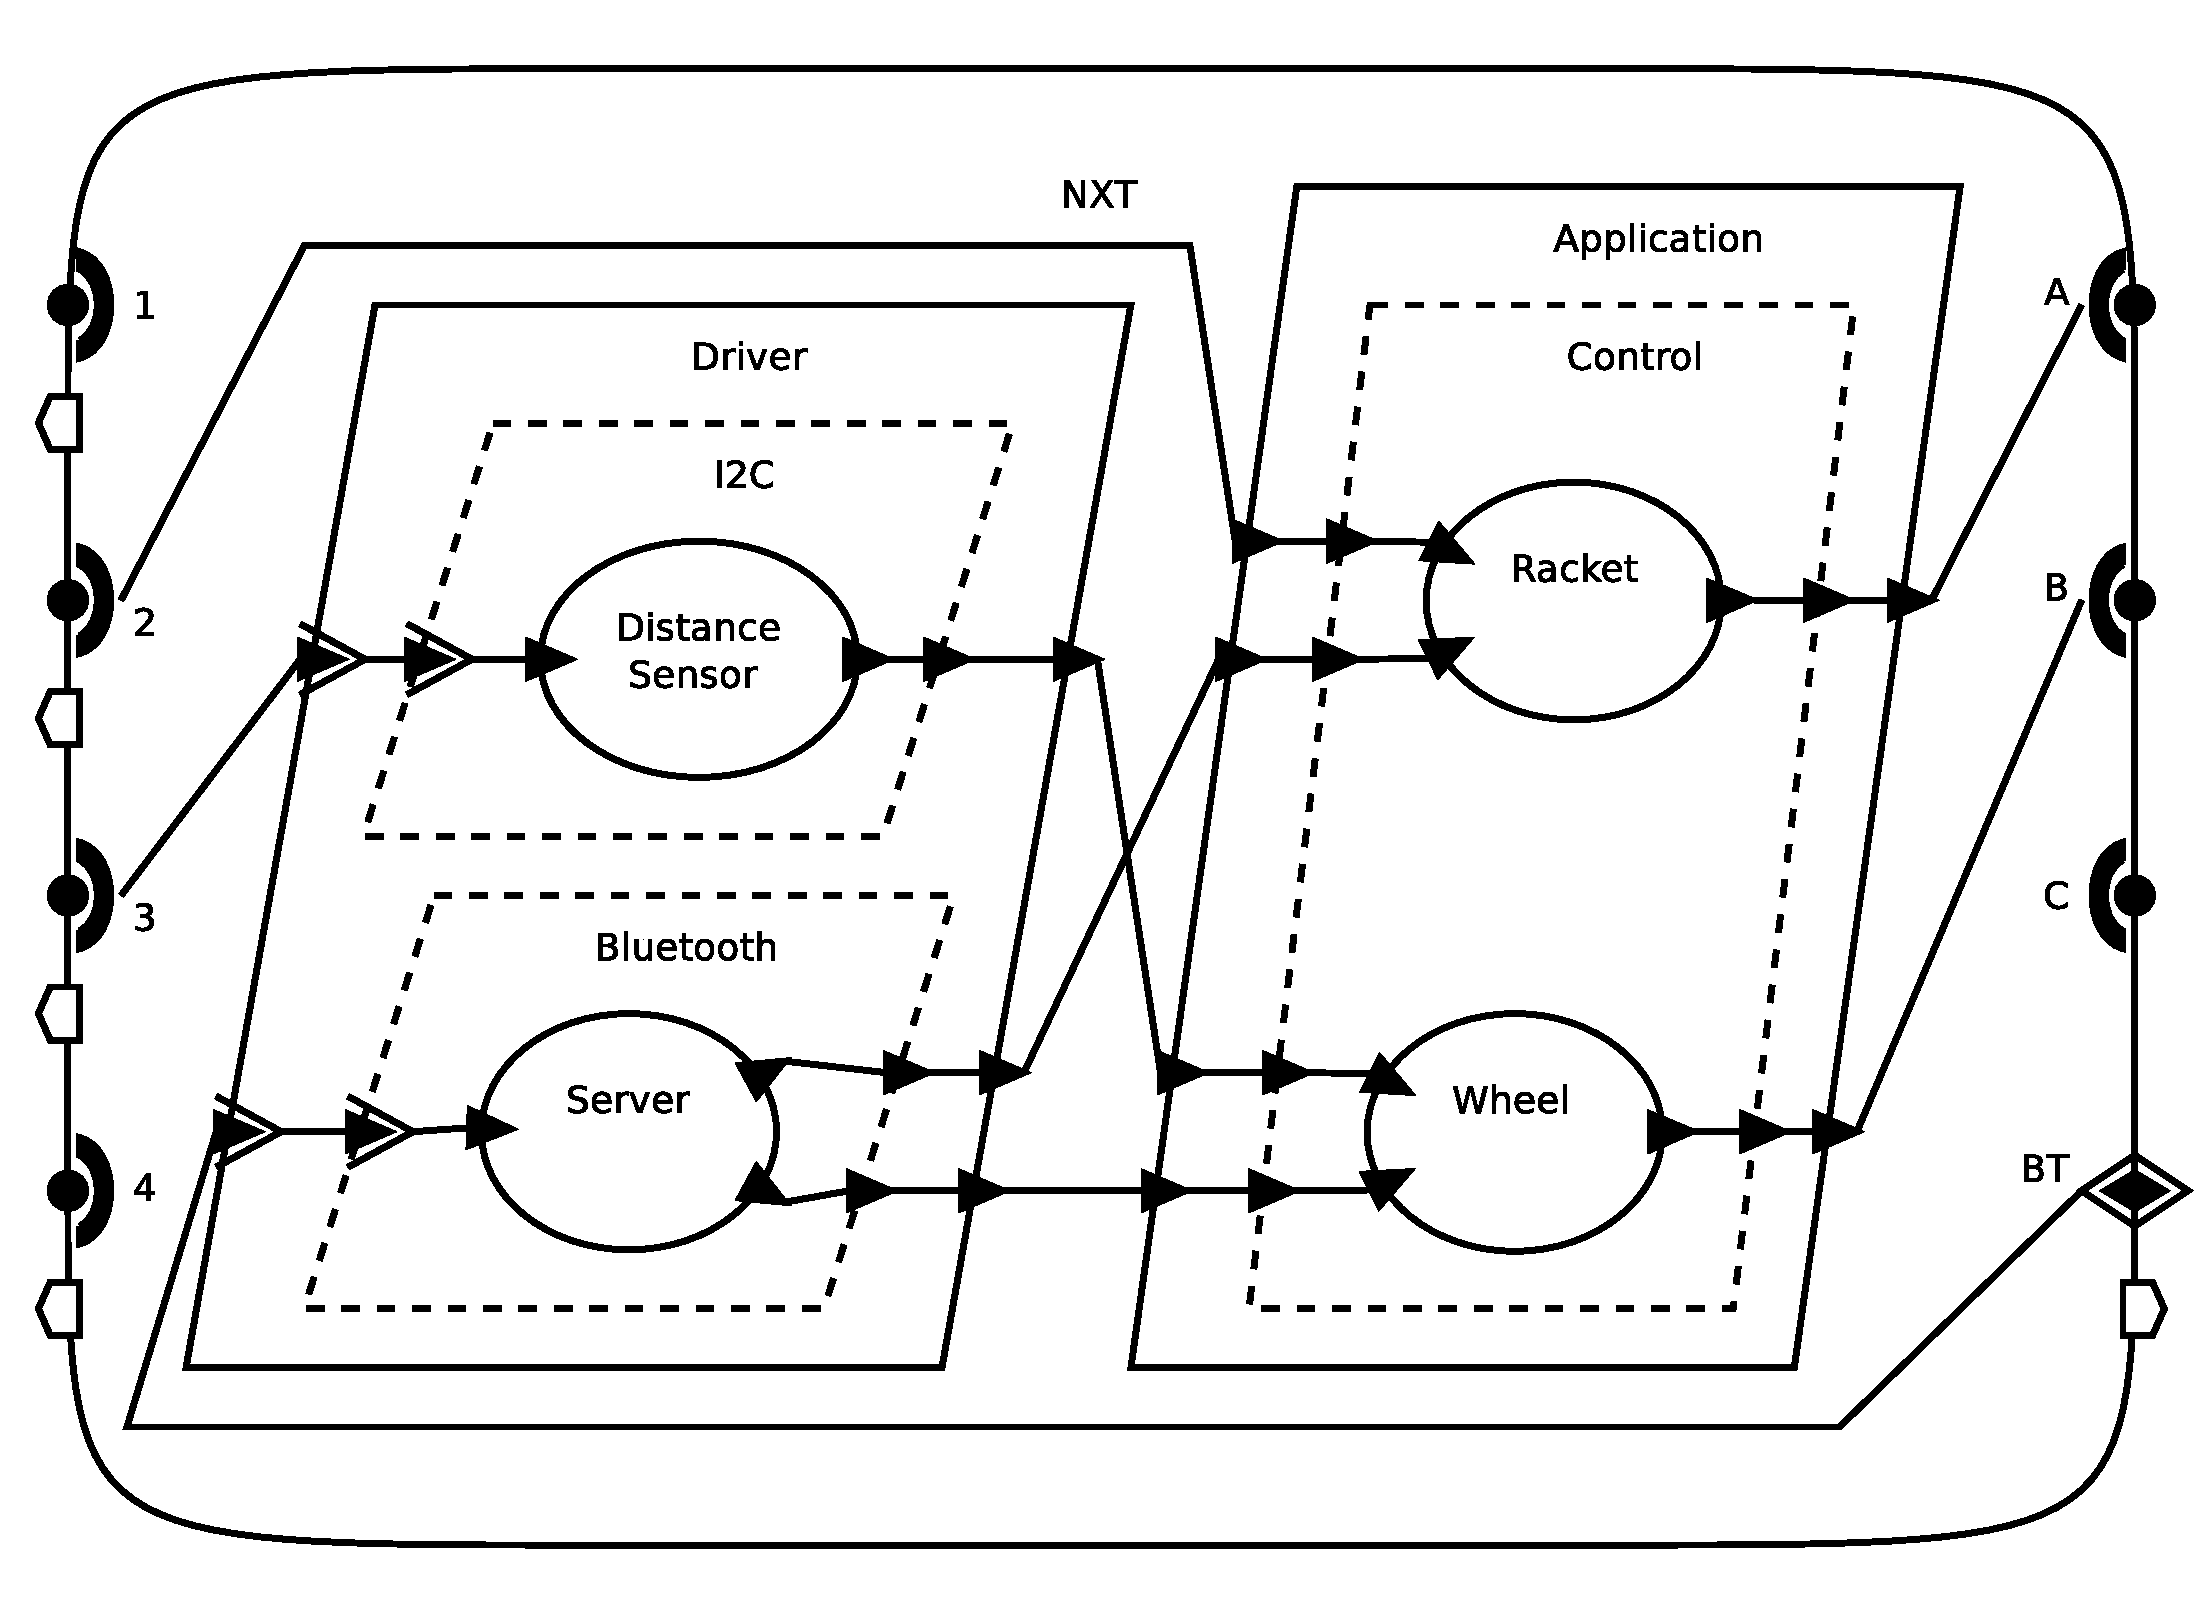
\includegraphics[scale=0.25]{./img/aadl-nxt1s.pdf}
        \caption{Modélisation AADL des composants logiciels du NXT.}
        \label{fig:aadl-nxt1s}
      \end{figure}

      La figure \ref{fig:aadl-nxt1s} offre une représentation graphique du
      modèle logiciel interne du {\it NXT}. Il est constitué de deux processus.
      Le premier processus ({\it Driver}) regroupe les pilotes de périphériques,
      il est composé d'une tâche pour le pilote {\it I2C} et d'une autre tâche
      pour le pilote {\it bluetooth}. Le seconde processus ({\it Application})
      contient la tâche d'asservissement du robot ({\it Control}).

      Le flux des données {\it bluetooth} lie le port d'entrée/sortie
      {\it BT} au processus regroupant les pilotes puis à la tâche du
      pilote {\it bluetooth}. Les données y sont traitées puis
      envoyées vers la tâche d'asservissement. Le flux des données
      {\it I2C} lie le groupe de ports {\it 3} au processus regroupant
      les pilotes puis à la tâche du pilote {\it I2C}. De la même
      façon, les données y sont traitées puis envoyées vers la tâche
      d'asservissement.

      La tâche d'asservissement contient deux sous-programmes. Le premier ({\it
        Racket}) récupère une donnée sur la proximité de la balle issue du pilote
      {\it bluetooth} et une donnée sur la position de la raquette issue du
      groupe de port {\it 2} et défini une vitesse à donner au moteur de la
      raquette sur le groupe de ports {\it A}. Le second ({\it Wheel}) récupère
      une donnée sur la position de la balle issue du pilote {\it bluetooth} et
      une donnée sur la position du robot issue du pilote {\it I2C} et défini
      une vitesse à donner au moteur de la roue sur le groupe de ports {\it B}.

      \subsubsection{Seconde spécification}

      \begin{figure}[!ht]
        \centering
        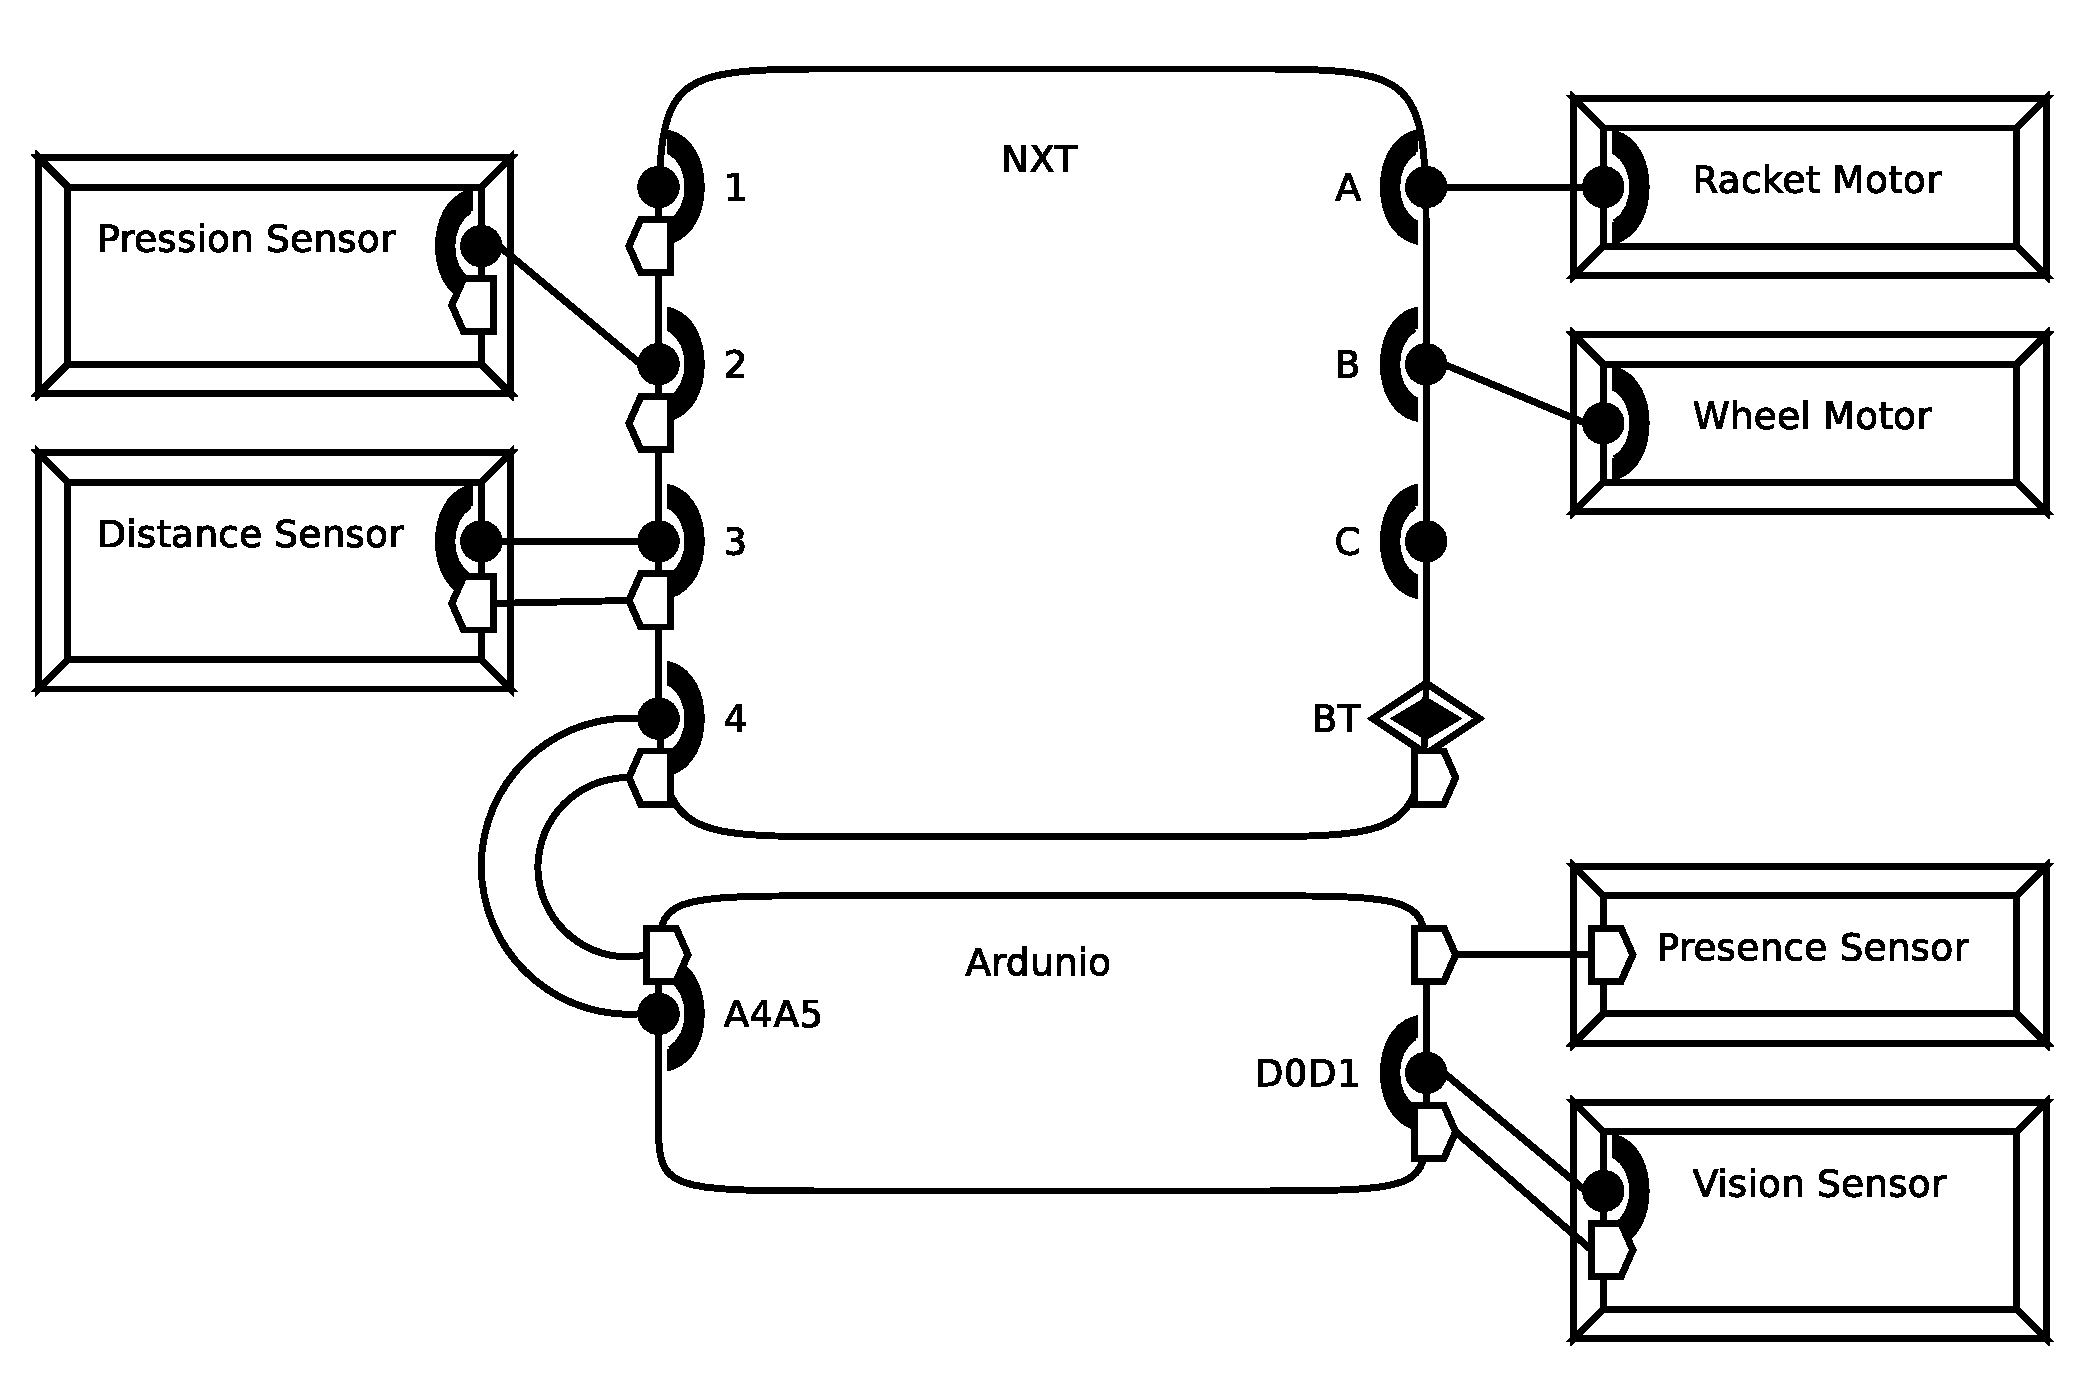
\includegraphics[scale=0.25]{./img/aadl-robot2.pdf}
        \caption{Vue global du système.}
        \label{fig:aadl-robot2}
      \end{figure}

      La figure \ref{fig:aadl-robot2} offre une représentation graphique du
      macro-modèle du robot suite à la modification de la spécification du
      démonstrateur. Celle-ci est semblable à la précédente à l'addition du
      système {\it Arduino} près. Le périphérique {\it bluetooth}, qui n'est
      plus utilisé, n'est plus représenté dans ce modèle.

      Afin de déterminer la position de la balle le système {\it
        Arduino} est couplé à deux périphérique. Une caméra ({\it Vision
        Sensor}) pour déterminer une position à distance du robot et une capteur
      de proximité ({\it Presence Sensor}) pour déterminer une position à
      proximité du robot. 

      Le flux de données et d'évènements entre la caméra et l'{\it Arduino} est
      réalisé par une connection sur un bus {\it UART}. Le capteur de proximité
      requiert un accès à une donnée interne à l'{\it Arduino}.  Le flux de
      données entre le système {\it Arduino} et le système {\it NXT} est réalisé
      par une connection sur le bus {\it I2C} du groupe de port {\it 4} dud
      système {\it NXT}.

      ~

      \begin{figure}[!ht]
        \centering
        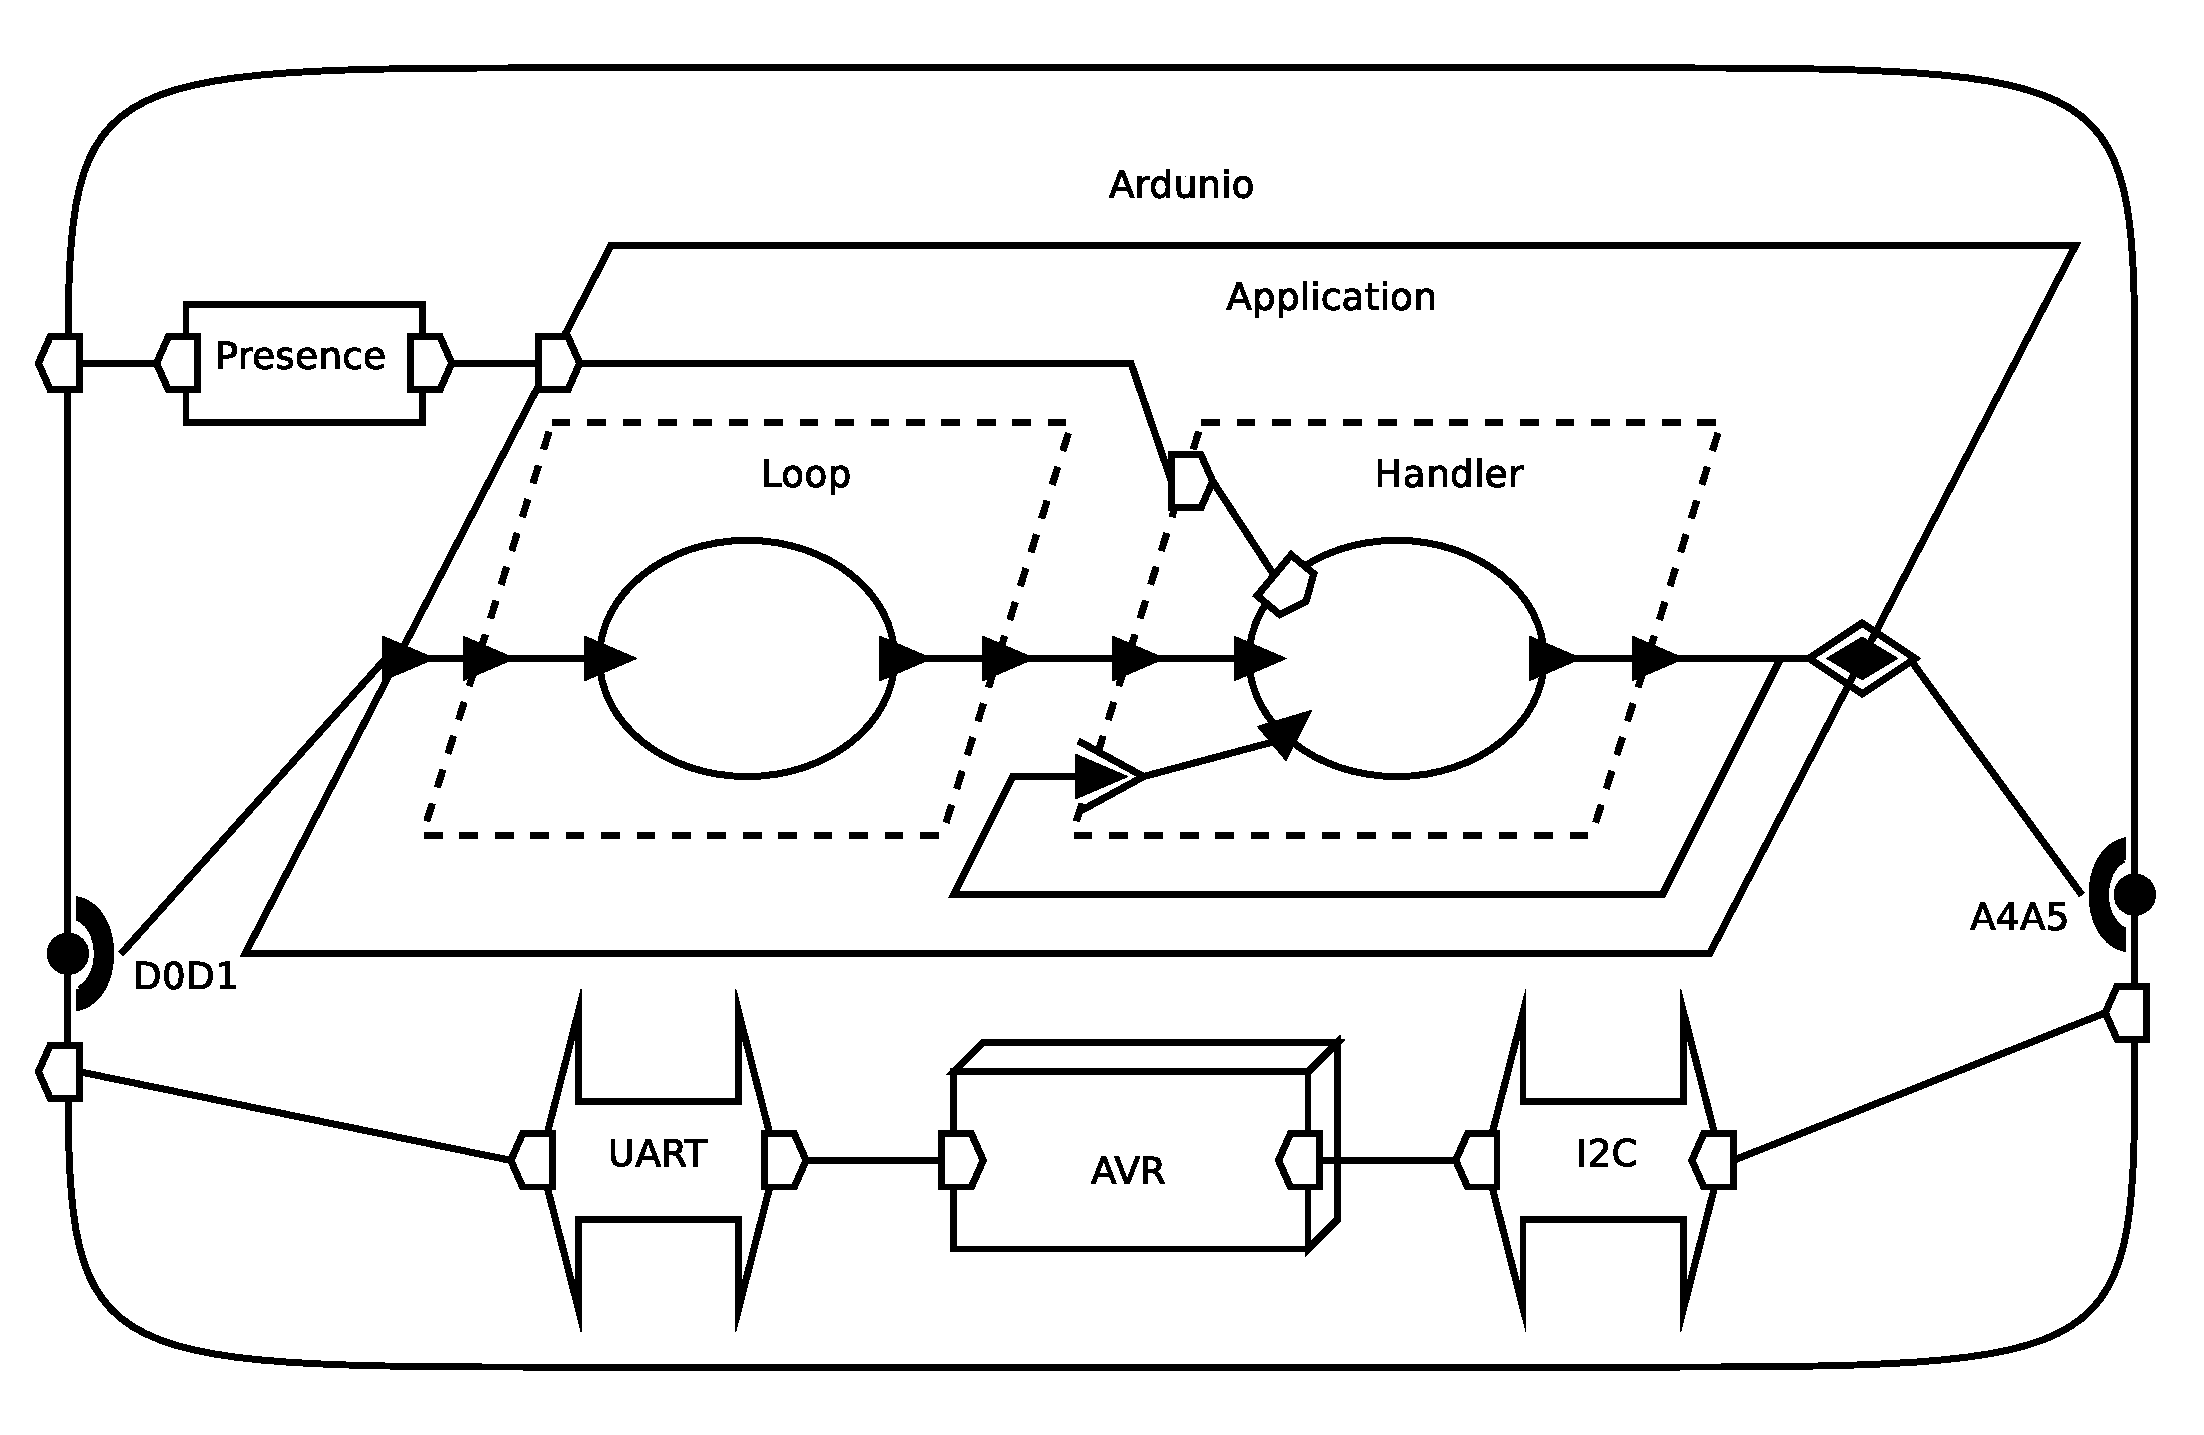
\includegraphics[scale=0.25]{./img/aadl-arduino.pdf}
        \caption{Modélisation AADL de l'Arduino.}
        \label{fig:aadl-arduino}
      \end{figure}
      
      La figure \ref{fig:aadl-arduino} offre une représentation graphique du
      modèle matériel et logiciel interne de l'{\it Arduino}. La composition
      matérielle de l'{\it Arduino} est relativement simple : il est constitué
      d'un microprocesseur {\it AVR} et de deux bus ({\it I2C} et {\it UART}).
      
      Il est constitué d'un processus ({\it Application}) reougroupant deux
      tâches. La première tâche ({\it Loop}) récupère les données issues de la
      caméra. La seonde tâche ({\it Handler}) est activée lorsqu'une requête est
      émise sur le bus {\it I2C}, elle retourne sur ce bus les données de la
      caméra et du capteur de proximité.
      
      ~

      \begin{figure}[!ht]
        \centering
        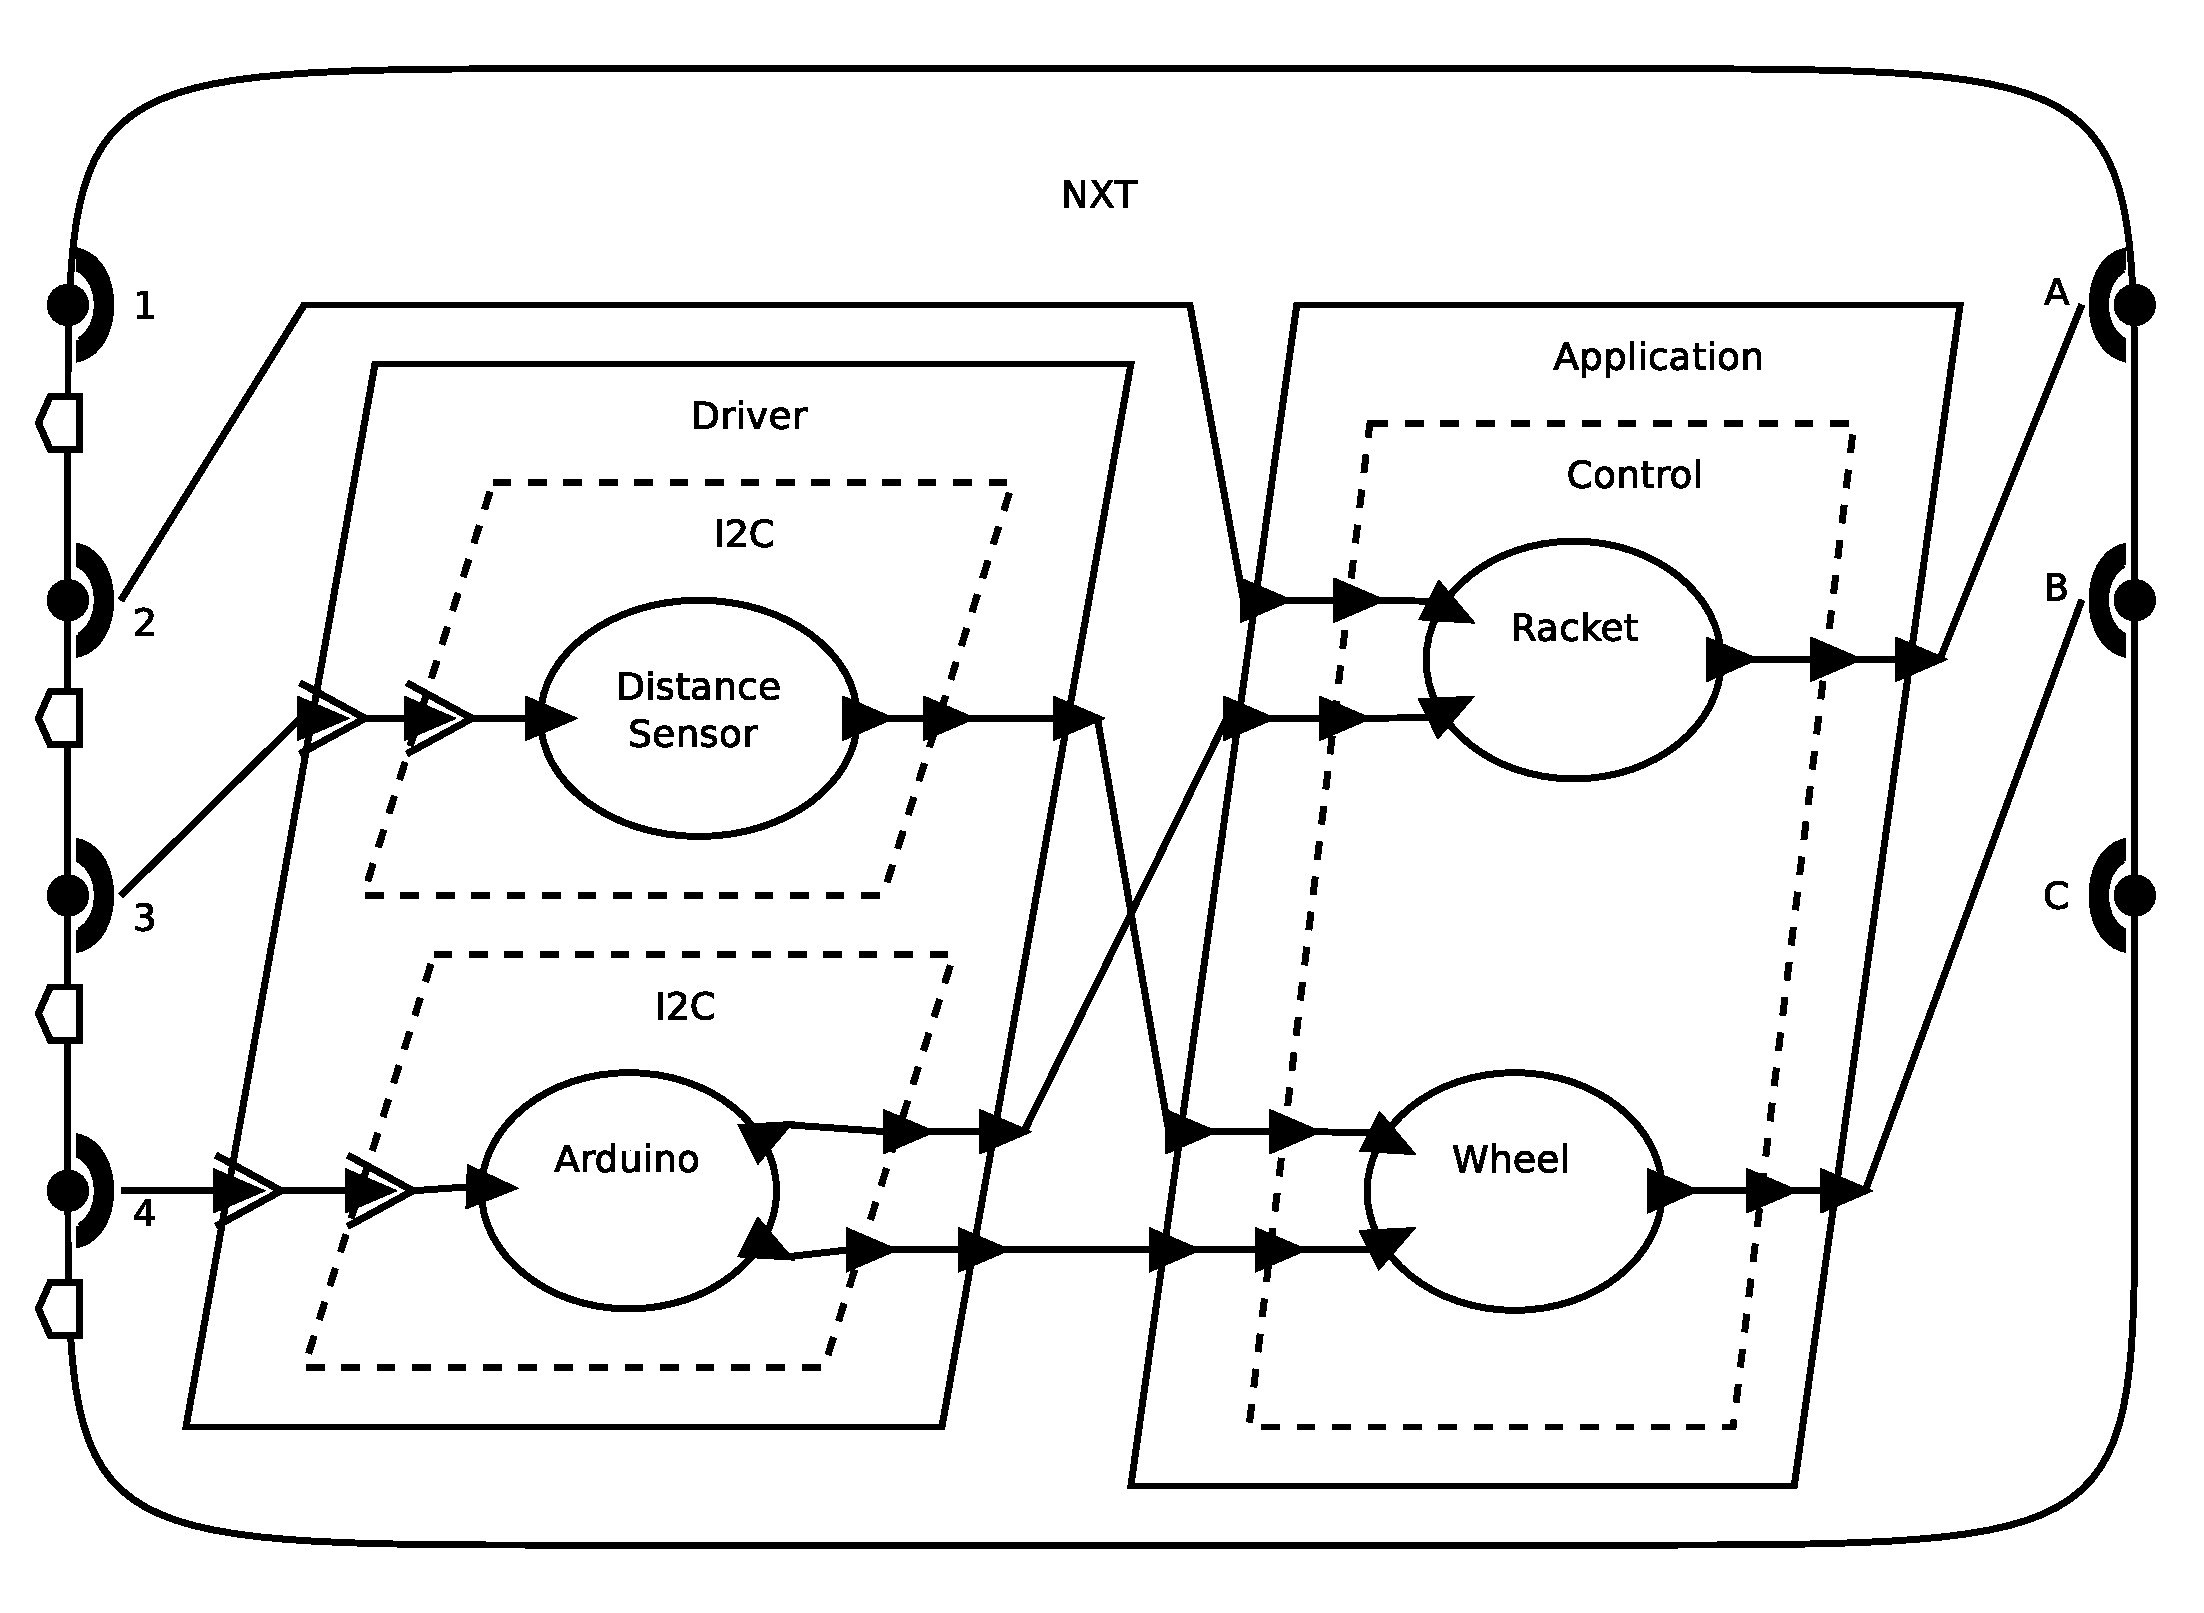
\includegraphics[scale=0.25]{./img/aadl-nxt2s.pdf}
        \caption{Modélisation AADL des composants logiciel du NXT.}
        \label{fig:aadl-nxt2s}
      \end{figure}

      La figure \ref{fig:aadl-nxt2s} offre une représentation graphique du
      modèle logiciel interne du {\it NXT}. De la même façon que dans le modèle
      correspondant de la première spécification il est constitué de deux
      processus. Le premier processus ({\it Driver}) regroupe les pilotes de
      périphériques, il est composé de deux tâches correspondant à deux
      instances du pilote {\it I2C}. Le seconde processus ({\it Application})
      contient la tâche d'asservissement du robot ({\it Control}).

      Le premier flux de données {\it I2C} lie le groupe de ports {\it 4} au
      processus regroupant les pilotes puis à l'instance du pilote {\it I2C}
      consacré à l'{\it Arduino}. Les données y sont traitées puis envoyées vers
      la tâche d'asservissement. Le second flux des données {\it I2C} lie le
      groupe de ports {\it 3} au processus regroupant les pilotes puis à
      l'instance du pilote {\it I2C} consacré au capteur de distance. De la même
      façon, les données y sont traitées puis envoyées vers la tâche
      d'asservissement.

      Le fonctionnement interne du second processus ({\it Application}) et
      sensiblement le même que dans le modèle correspondant de la première
      spécification. 
      
      ~

      Le travail de modélisation présenté ci-dessus présente partiellement le
      travail de modélisation réalisé. En effet, celui-ci a été produit dans le
      format textuel d'AADL. Il est en partie reproduit en annexe
      \ref{ann:aadl}, le travail complet étant accessible sous forme d'un projet
      Osate sur un dépot public\footnotemark. La modélisation produite a été
      validé par mes encadrants lors de différentes réunions de travail.
      \footnotetext{\url{http://github.com/LiberH/srsar/tree/master/models/aadl}}
      
      Il a été décidé de présenté ici certaines partie importante de ce travail
      de modélisation sous forme graphique de manière à être expliqué plus
      efficacement et compris plus facilement.
      
    \subsection{Modélisation comportementale}

      Afin de réaliser la modélisation comportementale c'est UPPAAL \cite{uppaal}
      qui a été choisi. UPPAAL, pour {\it Uppsala} et {\it Aalborg} les deux
      universités à l'origine de cet outil, est un environnement de modélisation
      pour le temps réel, les modèles manipulés sont réseaux automates temporisés.

      Le choix de cet outil résulte de plusieurs facteurs.  Le travail de
      modélisation attendu aurait pu être fait sous forme de réseaux de Petri et
      donc avec un autre outil, cependant, il m'a semblé plus naturel de le
      réaliser sous forme d'un réseaux d'automates temporisés. L'un des
      avantages de cet outil est son interface graphique qui intégre différents
      outils permetant de modéliser, simuler, et vérifier de manière simple et
      rapide le système considéré. Enfin, ayant déjà travaillé avec UPPAAL par
      le passé j'ai pu rapidement le reprendre en main.

      ~

      \begin{figure}[!ht]
        \centering
        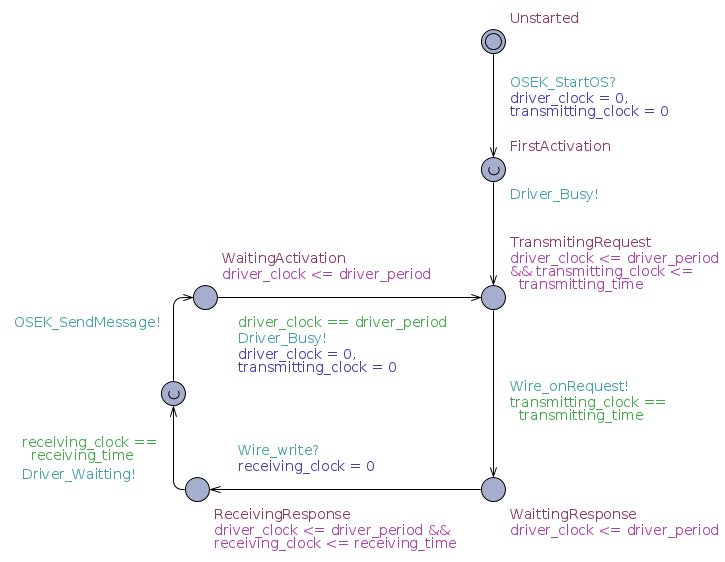
\includegraphics[scale=0.5]{./img/uppaal-driver.png}
        \caption{Modélisation de la tâche {\it I2C}}
        \label{uppaal-driver}
      \end{figure}
      
      
      La figure \ref{uppaal-driver} offre une représentation du modèle de la
      tâche {\it I2C} du NXT. Celle-ci joue le rôle de pilote de périphérique
      pour l'I2C.
      
      Initialement, l'état courant de
      l'automate est {\it Unstarted}. Un temps indéfini peut y être passé en
      attente du démarrage du système d'exploitation. Ce comportement est
      modélisé par la synchronisation de l'automate sur l'action
      {\it OSEK\_StartOS}. Lorsque le système d'exploitation démarre, l'action
      {\it OSEK\_StartOS} est réalisée, la transition est prise. L'automate
      se trouve alors dans l'état {\it FirstActivation}. Cet état est dit
      {\it urgent}, cela signifie que que la transition sortant de cet état
      sera prise dès qu'elle pourra l'être. Par construction, cette dernière l'est
      immédiatement, l'action {\it Driver\_Busy} est alors réalisée.
      Ce comportement modélise l'activation de la tâche {\it I2C} au démarrage
      du système d'exploitation.
      
      Cette tâche étant périodique, le modèle est contraint de ne jamais
      s'exécuter plus longtemps que sa période. Cela est modélisé par
      l'utilisation d'invariants ({\tt driver\_clock <= driver\_period}).
      
      ~
      
      Le nouvel état courant est {\it TransmitingRequest}. L'automate temporisé
      décrit une boucle modélisant quatres actions sucessives retournant en cet état. La
      première action, réalisée dans l'état {\it TransmitingRequest}, est la
      transmission de la requête I2C sur le bus associé. Ce comportement n'est
      modélisé que par un temps car le bus I2C est déterministe et son débit
      est connu. Il est donc possible de déterminer précisemment le temps que
      cette transmission prend. Une fois ce temps écoulé, l'action {\it Wire\_onRequest}
      est réalisée et l'état courant devient {\it WaitingResponse}.
      
      La seconde action, modélisée par un écoulement de temps dans ce nouvel état, est
      l'attente de la réponse du périphérique I2C. L'automate se synchronise
      alors sur l'action {\it Wire\_write} indiquant le début de la transmission de la réponse du
      périphérique. Une fois cette action réalisée, le nouvel état courant est
      {\it ReceveingResponse}.
      
      Cet état modélise la transmission de la réponse sur le bus I2C. De même
      que pour la transmission précédente, il est possible d'en connaitre exactement
      le temps d'exécution. Cette action n'est donc modélisée que par une attente. Une fois
      ce délai écoulé le pilote utilise une primitive du système d'exploitation
      pour envoyer un message à la tâche concernée ({\it Control}). Une fois ce
      message reçu par la tâche {\it Control}, l'état courant du pilote I2C est
      {\it WaitingActivation}.
      
      Dans cet état, c'est l'attente de l'échéance de la période qui est
      modélisée. Une fois cette attente terminée, le cycle reprend depuis l'état
      {\it TransmittingRequest}.
      
      ~

      \begin{figure}[!ht]
        \centering
        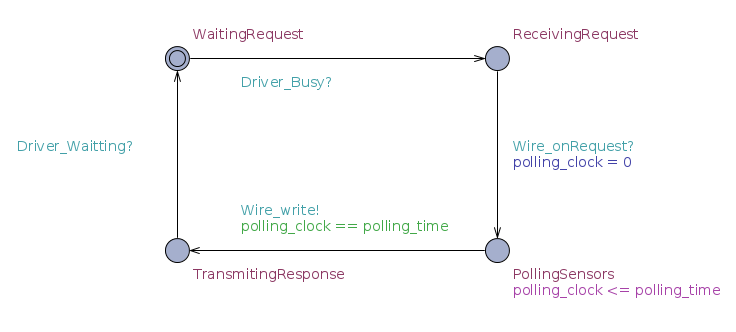
\includegraphics[scale=0.5]{./img/uppaal-handler.png}
        \caption{Modélisation de la tâche {\it Handler}}
        \label{uppaal-handler}
      \end{figure}


      La figure \ref{uppaal-handler} offre une représentation du modèle de la
      tâche {\it Handler} de l'Arduino. L'état initial de cet automate est
      {\it WaitingRequest}. Cette tâche est activée sur reception
      d'une interruption. Ce comportement est modélisé par une synchronisation
      sur action de mise en fonctionnement du pilote {\it I2C} du NXT
      ({\it Driver\_Busy}). L'état courant de l'automate est alors
      {\it ReceivingRequest}, un temps indéfini s'écoule dans cet état. C'est le
      temps de transmission de la requête évoquée dans la description du modèle
      du pilote I2C ci-dessus. Une fois ce temps écoulé, l'action
      {\it Wire\_onRequest} est réalisée par le pilote I2C, la transition est
      donc franchie dans cet automate et son état courant devient
      {\it PollingSensors}.
      
      Dans cet état l'Arduino interroge ses périphériques et construit la
      réponse à la requête I2C qu'il vient de recevoir. Une fois construite, il
      réalise l'action {\it Wire\_write} et débute la transmission de sa
      réponse vers le NXT. Son nouvel état courant est {\it TransmittingResponse}.
      
      À l'image du comportement observé dans l'état {\it ReceivingRequest}, il
      s'y écoule un temps défini dans le modèle du pilote I2C à la fin duquel
      le pilote réalise l'action {\it Driver\_Waiting}. Le nouvel état de
      l'automate est alors {\it WaitingRequest}. Le cycle reprend comme décrit
      ci-dessus.

      ~
      
      Le travail de modélisation décrit ici ne présente que partiellement le
      travail de modélisation réalisé. Les autres modèles réalisés sont reproduits en annexe
      \ref{ann:uppaal}. Le travail complet est accessible sous forme d'un projet
      UPPAAL sur un dépot public\footnotemark. La modélisation produite a été
      validée par mes encadrants lors de différentes réunions de travail.
      \footnotetext{\url{http://github.com/LiberH/srsar/tree/master/models/uppaal}}
      
      ~

      Lors de la production de ces modèles certaines problèmatiques ont été
      rencontrées. Par exemple, une question a été soulevée autour de la
      modélisation d'actions prennant un temps infime -- vis-à-vis des autres temps
      modélisés. Ne pas modéliser ces temps peut induire des comportements
      Zénon. Cependant, les modéliser implique soit de les modéliser plus grand
      qu'ils ne sont réellement, soit d'induire un écart important entre
      les plus petit et les plus grand temps modélisé. Cette dernière option a
      des conséquences significativement négatives sur l'efficacité des
      vérifications à réaliser sur le modèle considéré.
                  
      ~
      
      L'ensemble du comportement du démontrateur n'as pas été modélisé.
      En effet, les dynamiques de la balle et du moteur entrainant la roue ne sont pas
      modélisées. En l'état, s'il est possible de savoir si le robot frappe la
      balle lorsque celle-ci est à sa portée, il n'est cependant pas possible de
      savoir si le robot est effectivement placé en face de la balle lorsqu'il
      le fait.
      
      De telles dynamiques posent ici un problème de modélisation. En effet, elles
      ne peuvent pas être précisement modélisées par des modèles discrets. Or,
      les automates temporisés font parties de cette classe de modèles.
      Une solution peut être de discrétiser ces dynamiques. Cependant, cela
      implique une modélisation aproximée de la réalité et qui pourrait en être
      trop éloignée. Une autre solution évoquée au cours d'une réunion de travail
      est non-plus de modéliser la dynamique de la balle mais de réaliser un
      modèle statistique de la position de celle-ci.
      
  \section{Implémentation}
      
      Il était initiallement prévu que le démonstrateur soit fonctionnel avant
      le commencement de ce stage. Cependant, certains imprévus ayant fait
      contre-temps ont empêchés de produire le travail nécessaire sur le
      démonstrateur. Il était cependant nécessaire d'avoir un support sur lequel réaliser mes
      travaux. J'ai donc repris le travail de réalisation du démonstrateur,
      ce qui a partiellement modifié la nature de mon travail.
      
      ~
      
      La réalisation de cette implémentation a été chronophage et à
      ralenti mon travail vis-à-vis de ses objectifs initiaux. En effet,
      certains problèmes techniques, matériels comme logiciels, ont été
      rencontrés. Cela, que ce soit autour des objectifs du stage qui s'est
      déroulé en parallèle au mien, qu'autour d'autres problèmatiques de
      l'implémentation du démonstrateur. De fait une part importante de mon
      temps à été consacré à ce travail.
  
    \subsection{Implémentation matérielle}
 
      Le robot NXT Mindstorm de Lego a été développé pour initier les jeunes
      adolescents à la robotique et à la programmation informatique. Il a vite
      était repéré et récupéré par des adultes passionnés d'électronique ou de
      robotique pour son utilisation simple pouvant être facilement
      étendue. Afin de permettre une utilisation facile de son jouet, Lego a
      conçu le Mindstorm NXT comme suit : il y a une ``brique intelligente'', ou
      brique principale, concentrant l'ensemble des composants électroniques
      formant le ``cerveau'' du robot. Celle-ci peut-être reliée en USB à un
      ordinateur pour y déposer un programme. Elle comporte un écran et des
      boutons permettant de déterminer quel programme on souhaite lancer lors de
      l'utilisation du système d'origine ou pour piloter une application en
      cours d'execution.

      ~
      
      \begin{figure}
        \centering
        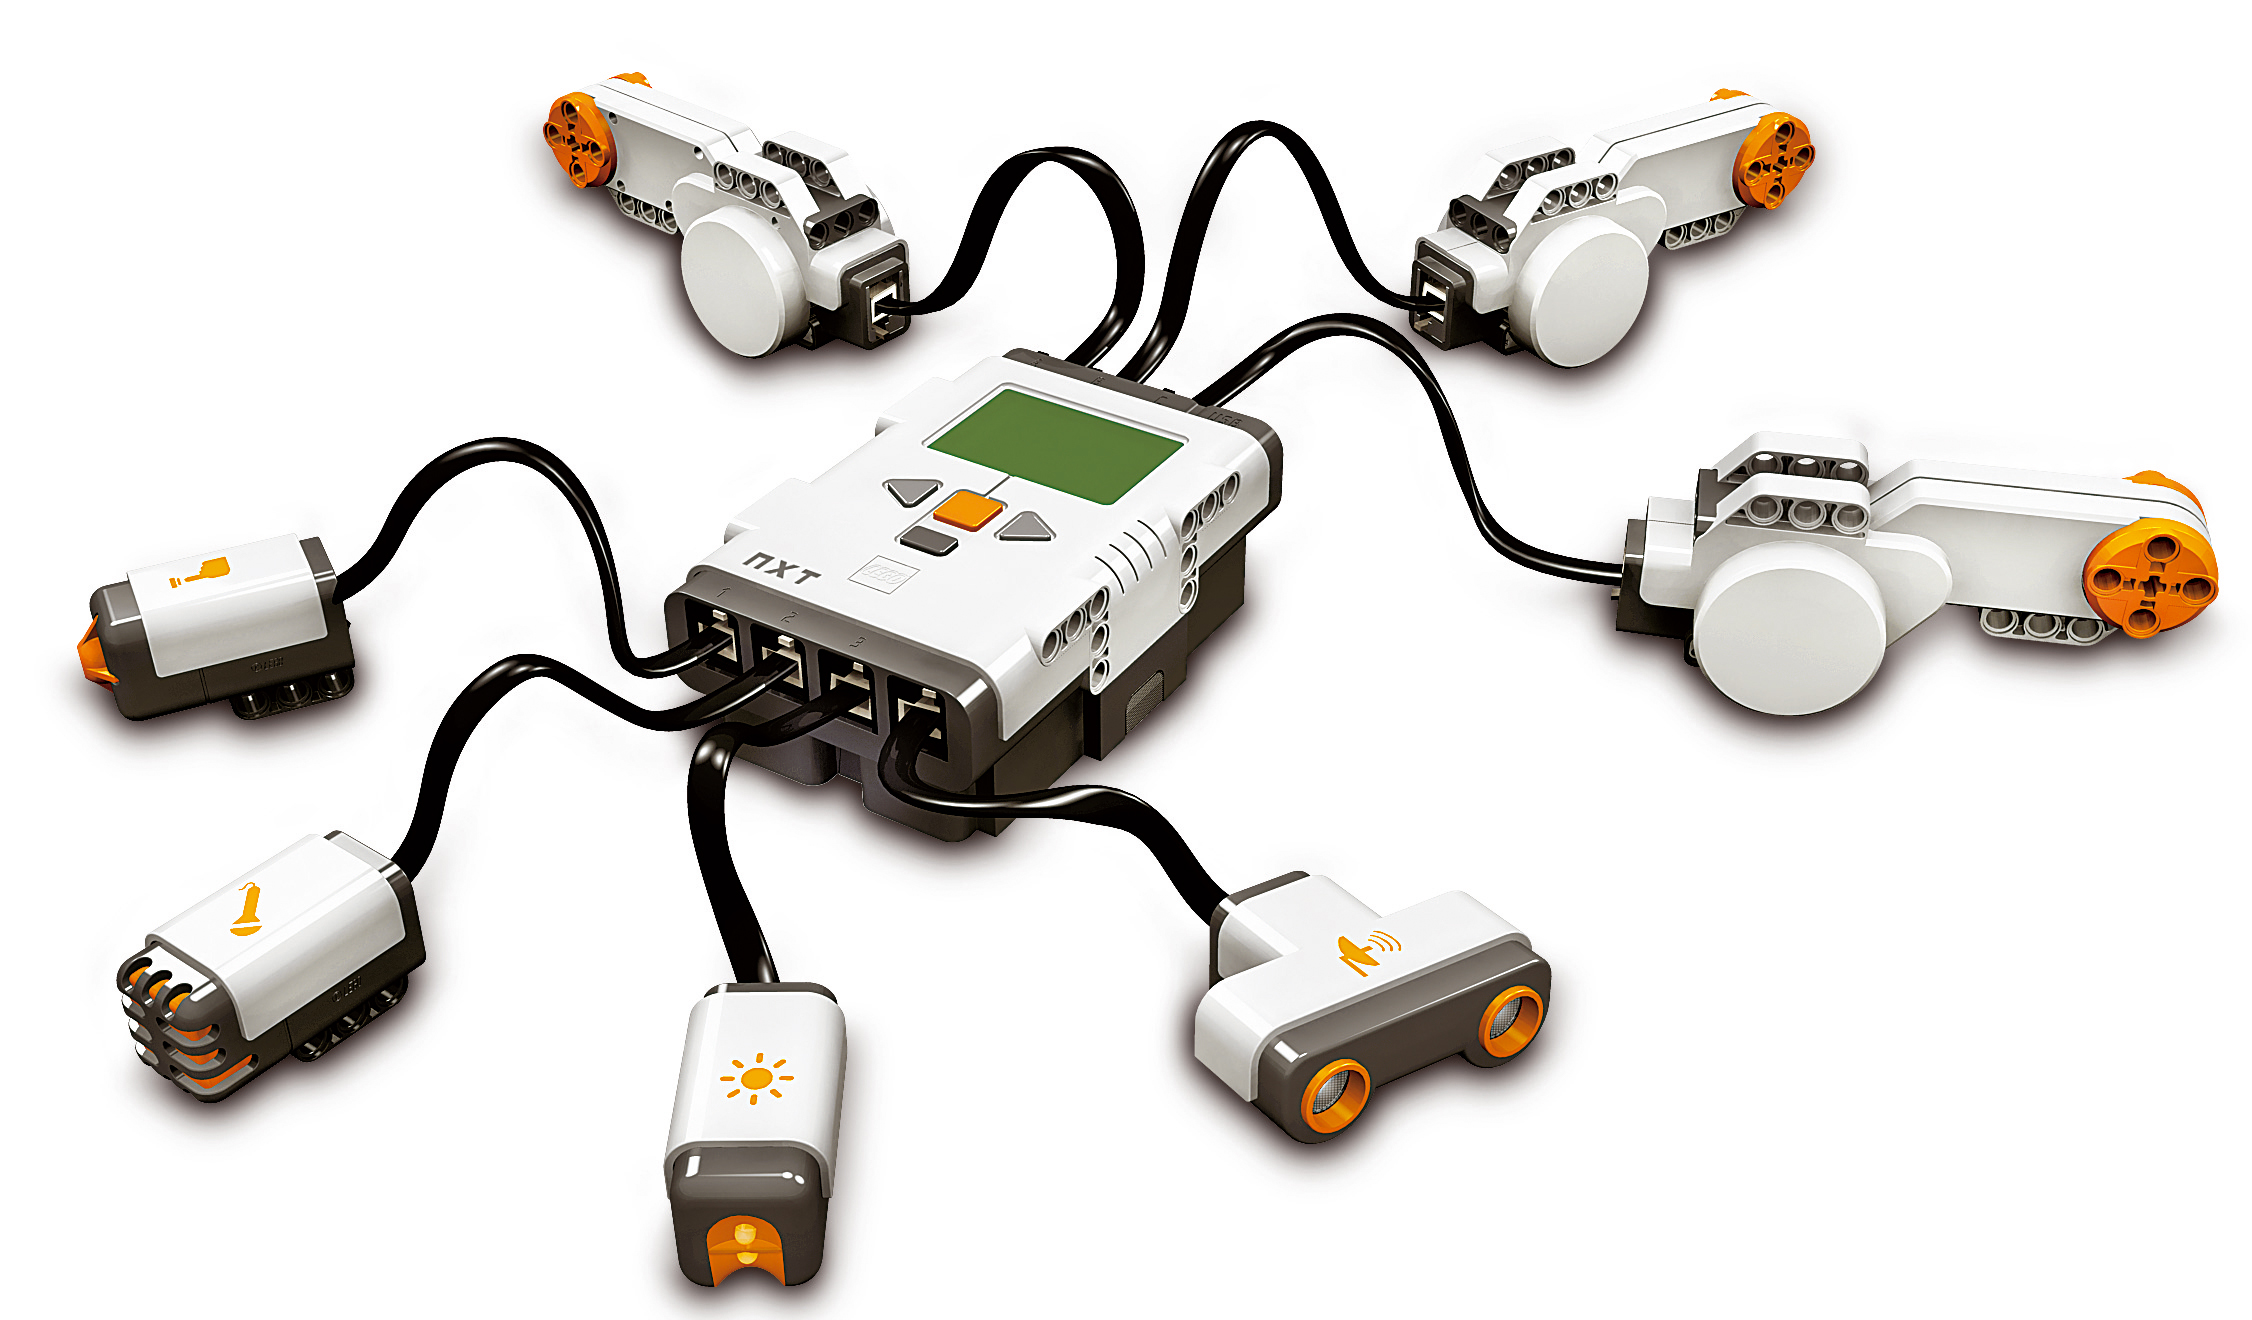
\includegraphics[scale=0.6]{./img/impl-nxt.jpg}
        \caption{Brique principale et périphériques du Minstorm NXT}
        \label{fig:impl-nxt}
      \end{figure}

      Sur cette brique peuvent être branchés des périphériques et plus
      précisemment 4 capteurs et 3 actionneurs. Leurs branchements sont
      facilités, utilisant tous les mêmes cables (RJ-12) comparables à des
      cables téléphoniques (RJ-11) -- voir figure \ref{fig:impl-nxt}. Mettant de
      côté les aspects complexes et fastidieux de la conception robotique,
      mécanique et électronique, il permet l'économie de leur mise en \oe uvre
      du point de vue du temps investi comme des moyens financiers
      engagés. C'est pour cet ensemble de raisons qu'il a été choisi le robot
      NXT en tant que composant intelligent du démonstrateur.

      ~
      
      \begin{figure}[!ht]
        \centering
        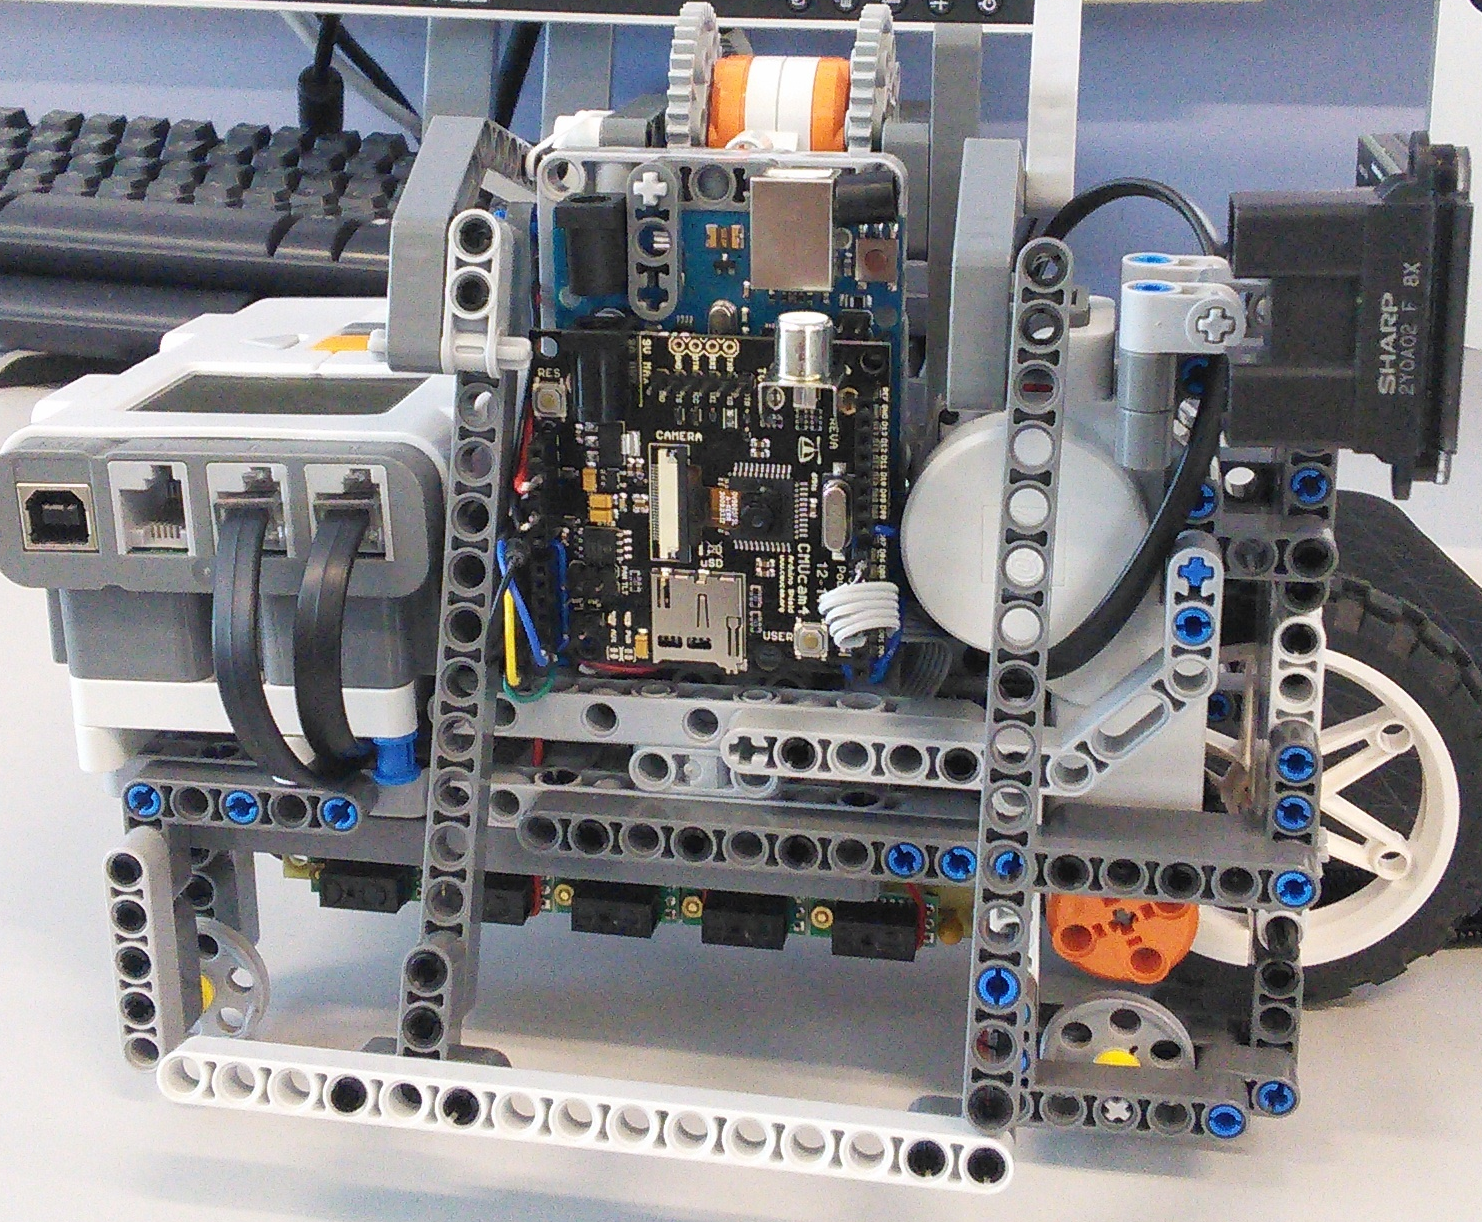
\includegraphics[width=0.8\textwidth]{./img/impl-robot.png}
        \caption{Une vue de l'implémentation matérielle du robot}
        \label{fig:impl-robot}
      \end{figure}
    
      Un second étudiant a travaillé sur l'implémentation matérielle du
      démonstrateur. Il a en effet participé à l'intégration de la caméra
      embarquée sur le robot NXT. Cette intégration a de fait modifié le
      démonstrateur -- voir figure \ref{fig:impl-robot}. Ces modifications ont
      été répércutées sur les différentes modélisations qui avaient été
      réalisées comme cela a pu être constaté ci-avant.

    \subsection{Implémentation logicielle}

      L'équipe Systèmes Temps Réel de l'IRCCyN travaille, entre autres choses,
      autour de ce qu'on appelle un système d'exploitation. C'est à dire une
      interface logicielle permettant d'abstraire l'utilisation des ressources
      matérielles -- électricité, espace mémoire, temps processeur, etc. -- d'un
      système physique. Le système d'exploitation que developpe l'équipe
      Systèmes Temps Réel a quelques particularités techniques le différenciant
      de celui que peut utiliser un ordinateur individuel standard.

      ~
    
      Ce système est conçu pour être utilisé sur des cartes électroniques ayant
      des usages plus restreints mais surtout plus spécifiques qu'un ordinateur
      personnel, étant lui capable de beaucoup de choses. Cette particularité en
      fait un système d'exploitation dit embarqué. L'informatique embarquée est
      présente dans les voitures, les trains, les avions mais aussi les
      téléphones intelligents très à la mode à notre époque. Au delà de ces
      exemples elle se cache dans beaucoup d'objets du quotidien. Cela en fait
      un enjeu majeur du point de vue économique mais aussi et peut-être avant
      tout pour le confort de vie de chacun à l'exemple de l'avion où l'embarqué
      est utile à assurer la sécurité de tous.

      ~
    
      Une autre spécificité de ce système est le fait qu'il soit temps réel. Le
      temps réel est une notion définissant un comportement particulier du
      système. Lorsque que l'on utilise un système temps réel on est assuré
      d'obtenir des résultats corrects dans des délais connus.

      ~
    
      Trampoline, le système developpé par l'équipe Temps Réel, fonctionne sur
      la plateforme Lego NXT ce qui permet une utilisation rapide et facile de
      ce dernier, que ce soit pour les chercheurs ou les étudiants.
      
  \section{Analyse}
    
    Afin de réaliser l'analyse de robustesse c'est Roméo \cite{gardey05}
    qui a été choisi. Roméo est un outil logiciel de vérification de modèles temporisés
    developpé au sein de l'équipe Système Temps Réel de l'IRCCyN. Il est utilisé pour
    vérifier des réseaux de Petri T-temporels. Il permet de mettre en \oe uvre
    des vérifications de modèles réalisant des synthèses de paramètres entiers
    bornés.

    C'est la vérsion 3.0$\alpha$ de Roméo qui a été utilisée. C'est une version
    en cours de développement. Certains problèmes ont été rencontrés lors
    de son utilisation retardant un peu l'obtention des premiers résultats.
    Cependant, ce travail a permis de tester cette nouvelle version de Roméo
    et d'en corriger certains petits défauts. Roméo étant une
    réalisation importante de l'équipe Système Temps Réel, le temps qui y est
    consacré n'est pour pas perdu.
    
    ~
    
    Une première étape nécessaire au travail d'analyse de la robustesse du
    modèle comportemental du démonstrateur est sa traduction vers un modèle
    équivalent manipulable par Roméo. Le modèle comportemental produit grace
    à UPPAAL est sous forme d'automates temporisés alors que Roméo manipule
    des modèles du type {\it Clock Transition System} \cite{lime12} (CTS) 
    adaptés à la vérification de réseaux de Petri T-temporels.
    
    La sémantique des automates temporisés définissent un écoulement du temps dans
    les localités qui le composent alors que dans les CTS définissent des intervales 
    de tirs sur les transitions qui les composent, à la manière des réseaux de
    Petri T-temporels.
    
    Le travail de traduction de modéle réalisé est reproduit en annexe
    \ref{ann:romeo}. Il est également disponible sur un dépot
    public\footnotemark. La modélisation produite a été
    validée par mes encadrants lors d'une réunion de travail.
    \footnotetext{\url{http://github.com/LiberH/srsar/tree/master/models/romeo}}
    
    ~
    
    Différentes propriétés ont été vérifiées sur ce modèle. Une première
    propriété a permis de s'assurer de l'absence d'interblocage dans celui-ci.
    Une seconde propriété à permis de monter une vivacité locale. Ainsi, on peut
    avancer que le service fourni par le pilote {\it I2C} (figure
    \ref{uppaal-driver}) est rendu infiniment souvent.
    
    Différentes synthèses de paramètres ont été réalisées avec ce modèle.
    Celles-ci ont été produite pour un paramètre et vérifiant la propriété
    d'absence d'interblocage. Les résultat obtenus nous indiquent, par exemple,
    que la période du pilote {\it I2C} fixé à 50 millisecondes peut être
    augementée ou diminuée de 10 millisecondes sans que la propriété d'absence
    d'interblocage ne soit invalidée.

    Ces résultats ne sont pas très significatifs quant à la la robustesse du
    modèle considéré. Ces synthèses constituent une analyse préliminaire de la
    robustesse du modèle du démonstrateur. Les résultats évoquées ont pu
    être obtenus sur un ordinateur de bureau. Cela autorise à penser que des
    synthèses de paramétres plus complexes pourront être réalisées 
    dans des temps acceptable quitte a utiliser pour cela une machine spécialisée.
         
    ~
    
    Des vérifications et synthèses de paramètres s'appuyant sur des propriétés
    quantitatives sont prévue à cours terme. L'ensemble des éléments nécessaires à leur
    réalisations sont aujroud'hui à disposition. Il est par exemple prévu de synthétisé un
    intervalle pour la période du pilote {\it I2C} vérifiant la propriété
    suivante : l'age des données collectées par l'Arduino sont traitées par le
    NXT avant une date fixée. Ce travail n'a pu être réalisé par manque de temps
    principalement dû aux divers problèmes liés à l'implémentation du
    démonstrateur.
    
    ~
    
    De la même façon, il n'a pas pu être produit d'analyse utilisant l'approche
    par réduction des automates temporisés implémenté dans l'outil Shrinktech \cite{sankur13}.
    Le travail à réaliser afin d'avoir à disposition tous les éléments nécessaires à cette
    analyse est plus important que dans le cas de l'utilisation de Roméo.
    En effet, il est nécessaire de prendre en main cet outil ainsi que sa syntaxe,
    de traduire le modèle comportemental vers celle-ci. Il est également
    nécessaire d'obtenir et de prendre en main l'outil Kronos \cite{yovine97}.
    En effet, l'outil Shrinktech est partiellement basé sur ce dernier.
    Shrinktech étant très récent et peu répendu, il peut ne pas avoir
    été testé extensivement. À la différence de l'utilisation de Roméo, ce
    travaille ne pourra être fait efficacement grace à une proximité direct
    avec l'auteur de l'outil.

  \section{Bilan}

    Ce document est organisé de manière à expliquer simplement le
    travail produit. Il évoque tout d'abord le travail de modélisation réalisé puis le
    travail d'implémentation produit et enfin le travail de vérification et d'analyse
    de robustesse entamé. Cependant, la production de ces travaux n'a pas été réalisée dans ce même
    ordre. Il a été nécesaire de réaliser l'implémentation matérielle et
    logicielle afin d'en modéliser l'architecture et le comportement.
    L'évolution de la spécification du démonstrateur et les contre-temps liés
    à son implémentation ont impactés sur le travail de modélisation et
    repoussé dans le temps le réalisation de l'analyse de robustesse du
    démonstrateur.
    
    ~
    
    La travail attendu quant à l'implémentation et la modélisation a été
    réalisé. Et il est envisageable à court terme de réaliser l'analyse de
    robustesse du démonstrateur.
    
    Dans le cadre de projets aux thématiques proches de celles étudiées par le
    projet ImpRo, il est prévu de poursuivre le développement du démonstrateur.
    Il est prévu de produire une implémentation matérielle à partir d'autres
    matériaux que les Lego Technics utilisés à ce jour. Lors d'utilisations
    prolongées des robots, les pièces Lego finissent par connaitre du jeu mécanique, voire
    parfois par se détacher les unes des autres.
    Il est également prévus de mettre au propre et compléter l'implémentation 
    logicielle afin qu'elle puisse être facilement réutilisée.
    
    Il est évoqué comme objectif à long terme de générer tout ou partie de
    l'implémentation logicielle des robots du démonstrateur afin d'assurer une
    distance minimale entre les modèles considérés et les implémentations qui
    en sont faites. 
    
    ~

    Lors de l'écriture du rapport bibliographique j'ai réalisé un travail de
    recherche. J'ai en effet produit une synthèse de littérature scientifique
    dans le domaine des modèles temporisés. Pour une part avec des travaux
    definissant les bases téoriques du domaine et pour autre part avec des
    travaus de l'état de l'art concernant la robustesse des modèles temporisés.

    ~

    Lors de la modélisation du démonstrateur j'ai réalisé un travail de
    conception et d'analyse. J'ai en effet produit un modèle architectural du
    démonstrateur grace au langage de conception d'architectures des systèmes
    embarqués et temps réel AADL. De même, j'ai produit un modèle comportemental du
    démonstrateur grace à l'outil de modélisation d'automates temporisés
    UPPAAL. J'ai traduit ce modèle sous une forme proche des réseaux de Petri
    afin d'en réaliser une analyse avec l'outil de vérification Roméo.

    ~

    Lors de l'implémentaion du démonstrateur j'ai également réalisé un travail
    technique. J'ai en effet participé à l'implémentation
    matérielle du démonstrateur mettant en \oe uvre des compétences en
    électronique et en moindre mesure en mécanique. De même, j'ai participé à
    l'implémentation logicielle du démonstrateur mettant en \oe uvre des
    compétences en programmation bas niveau, temps réel et en système.

    ~

    À travers la réalisation de ce stage j'ai pu mettre en \oe uvre différentes
    compétences acquisent au fils de mon cursus scolaire. Ce faisant, j'ai
    également pu consolider mais connaissances théoriques et mes compétences
    pratiques.

    Sur certains aspects de ce stage j'ai travaillé en autonomie. Cela m'a
    permis de mettre en place une organisation de mon travail personnel. Sur
    d'autres aspects j'ai pu collaboré avec un autre stagiaire ou avec mes
    encadrants.

    J'ai également été confronté à des contraintes techniques et des
    contre-temps. En accord avec mes encadrants, il m'a fallu faire des choix
    pour dépasser ceux-ci. Il m'a également fallu comprendre que cela peut être
    le déroulement normal de ce type de mission.

